\documentclass{beamer}

\usepackage{beamerthemesplit}
\usepackage{verbatim}
\usepackage[normalem]{ulem}
\usepackage[caption=false]{subfig}
%\usepackage{tabularx}
%\usepackage{booktabs}



\usepackage{xcolor}

\usepackage{hyperref}

\definecolor{gold}{rgb}{1.,0.84,0.}
\definecolor{brightred}{rgb}{1.,0.4,0.4}
\definecolor{mygray}{RGB}{200,200,200}
\definecolor{lightsteelblue}{RGB}{176,196,222}
\definecolor{lightskyblue}{RGB}{135,206,250}
\definecolor{cadetblue}{RGB}{95,158,160}

\usetheme{default}
\usecolortheme{mule}

\usefonttheme{serif}

%\DeclareGraphicsExtensions{.pdf,.png,.jpg}

\newcommand{\mcal}{\textsc{metacalibration}}
\newcommand{\Mcal}{\textsc{Metacalibration}}

\newcommand{\mcalR}{\mbox{\boldmath $R$}}
\newcommand{\mcalRscalar}{\mbox{$R$}}

\newcommand{\mcalRmean}{\mbox{\boldmath $\langle R \rangle$}}
\newcommand{\mcalRscalarmean}{\mbox{$\langle R \rangle$}}

\newcommand{\mcalRpsf}{$R^{p}$}
\newcommand{\mcalRpsfnoise}{$R^{p}_\eta$}
\newcommand{\mcalRo}{\mbox{\boldmath $R_o$}}
\newcommand{\mcalRnoise}{\mbox{\boldmath $R_\eta$}}

\newcommand{\mcalRmeanalpha}{\mbox{\boldmath $\langle R_\alpha \rangle$}}
\newcommand{\mcalRmeanbeta}{\mbox{\boldmath $\langle R_\beta \rangle$}}

\newcommand{\mcalRg}{\mbox{\boldmath $R_\gamma$}}
\newcommand{\mcalRS}{\mbox{\boldmath $R_S$}}
\newcommand{\mcalRgmean}{\mbox{\boldmath $\langle R_\gamma \rangle$}}
\newcommand{\mcalRSmean}{\mbox{\boldmath $\langle R_S \rangle$}}

\newcommand{\mcalRtwopt}{\mbox{\boldmath $R^{2pt}$}}
\newcommand{\mcalRtwoptmean}{\mbox{\boldmath $\langle R^{2pt} \rangle$}}


\newcommand{\mcalRmodel}{\mbox{\boldmath $R^{model}$}}
\newcommand{\mcalRnoisemodel}{\mbox{\boldmath $R^{model}_\eta$}}


\newcommand{\vecg}{\mbox{\boldmath $\gamma$}}
\newcommand{\vest}{\mbox{\boldmath $e$}}

\newcommand{\snr}{$S/N$}
\newcommand{\snT}{$(S/N)_{\textrm{size}}$}
%\newcommand{\snT}{$\left( \frac{S}{N}\right)_{\textrm{size}}$}
\newcommand{\snflux}{$(S/N)_{\textrm{flux}}$}
%\newcommand{\snflux}{$\left( \frac{S}{N}\right)_{\textrm{flux}}$}
\newcommand{\hlr}{$r_{50}$}

\newcommand{\neff}{$n_{eff}$}

\newcommand{\lensfit}{\texttt{LENSFIT}}
\newcommand{\numba}{\texttt{Numba}}
\newcommand{\python}{\texttt{Python}}
\newcommand{\ngmix}{\texttt{ngmix}}
\newcommand{\ngmixer}{\texttt{ngmixer}}
\newcommand{\shear}{{\bf g}}
\newcommand{\redmapper}{redMaPPer}
\newcommand{\est}{$e$}


\newcommand{\prelim}{{\bf{\it Preliminary}}}

\newcommand{\uberseg}{{\color{lightsteelblue} {\"u}berseg}}
\newcommand{\MOF}{{\color{brightred}MOF}}


\title{Shear-dependent Detection Biases}
\author{Erin Sheldon}
\institute{Brookhaven National Laboratory}

% http://texblog.net/latex-archive/plaintex/beamer-footline-frame-number/
% to add the page (frame ) number and not screw up the bottom line
% works for split themes?
\expandafter\def\expandafter\insertshorttitle\expandafter{%
      \insertshorttitle\hfill%
        \insertframenumber\,/\,\inserttotalframenumber}

% suppress navigation bar
\beamertemplatenavigationsymbolsempty
\setbeamertemplate{footline}{}

\begin{document}

\usebackgroundtemplate{%
\includegraphics[width=\paperwidth]{hsc-firstpublicd.png}
}
\frame
{
}

%\setbeamertemplate{background canvas}[vertical shading][bottom=mgray,top=mblack]

%\setbeamerfont*{itemize/enumerate body}{size=\Large}
%\setbeamerfont*{itemize/enumerate subbody}{parent=itemize/enumerate body}
%\setbeamerfont*{itemize/enumerate subsubbody}{parent=itemize/enumerate body}


\frame{\titlepage}

\setbeamertemplate{background canvas}[vertical shading][bottom=mgray,top=mblack]

\setbeamerfont*{itemize/enumerate body}{size=\Large}
\setbeamerfont*{itemize/enumerate subbody}{parent=itemize/enumerate body}
\setbeamerfont*{itemize/enumerate subsubbody}{parent=itemize/enumerate body}




\frame
{
    \frametitle{Outline}

    \begin{itemize}

        \item Detection and Deblending
        \item Shear measurement tests with pairs of galaxies
        \item More realistic tests
        \item Mitigating detection bias with \mcal.
        \item Prospects for LSST

    \end{itemize}

}

\frame
{
    \frametitle{Detection and Deblending}

    \setbeamerfont*{itemize/enumerate body}{size=\small}
    \setbeamerfont*{itemize/enumerate subbody}{parent=itemize/enumerate body}
    \setbeamerfont*{itemize/enumerate subsubbody}{parent=itemize/enumerate body}
 
    \begin{itemize}

        \item By detection I mean the process of finding ``objects''.

        \item There are many different ways to do this, and it can include some
            kind of segmentation, as well as merging objects or splitting of
            objects at some level.

        \item By deblending I mean a second the stage of assigning light to the
            individual detections.

        \item In principle these can be combined, or the process could be iterative.

    \end{itemize}

}

\frame
{
    \frametitle{Tools used in this Work}

    \setbeamerfont*{itemize/enumerate body}{size=\normalsize}
    \setbeamerfont*{itemize/enumerate subbody}{parent=itemize/enumerate body}
    \setbeamerfont*{itemize/enumerate subsubbody}{parent=itemize/enumerate body}
 
    \begin{itemize}

        \item For all the tests I will show, detection was performed using SExtractor
            with the proposed settings for the final DES processing.

        \item All deblending is done as a second stage using a new implementation
            of the Multi-object Fitter (MOF) from DES. \url{https://github.com/esheldon/mof}

        \item All shear tests were performed using \mcal, which derives a shear
            calibration from the data itself using sheared versions of the images.
            \url{https://github.com/esheldon/ngmix}

    \end{itemize}

}


\frame
{
    \frametitle{Shear measurement tests with pairs of galaxies}

    \setbeamerfont*{itemize/enumerate body}{size=\normalsize}
    \setbeamerfont*{itemize/enumerate subbody}{parent=itemize/enumerate body}
    \setbeamerfont*{itemize/enumerate subsubbody}{parent=itemize/enumerate body}
 
    \begin{itemize}

        \item DES pixel scale (0.263'') and typcal seeing (0.9'')
        \item Generate images of two objects at fixed separation, but random
            relative position angle.

        \item Objects were bulge+disk with knots of star formation
            \begin{itemize}
                \item Bulge light fraction uniform random between 0 and 1
                \item Bulge and disk with different ellipticity.
                \item Bulge size different than disk.
                \item Bulge offset by up to 5\% of the half light radius \hlr.
                \item Knots followed the disk light, with as much as 20\%
                    of disk light in knots.
            \end{itemize}
        \item \snr\ for each object ranged between 20 and 40, so the objects
            are well above detection threshold

    \end{itemize}

}

\begin{frame}
    %\begin{block}{Results}
        \begin{figure}
            \begin{minipage}{.5\textwidth}
                \centering
                \subfloat[sep 4'']{\includegraphics[width=.475\linewidth]{{bdk-4.0as}.png}}~%
                \subfloat[sep 3'']{\includegraphics[width=.475\linewidth]{{bdk-3.0as}.png}}
            \end{minipage}%
            \begin{minipage}{.5\textwidth}
                \centering
                \subfloat[sep 2'']{\includegraphics[width=.475\linewidth]{{bdk-2.0as}.png}}~%
                \subfloat[sep 1.5'']{\includegraphics[width=.475\linewidth]{{bdk-1.5as}.png}}
            \end{minipage}\par\medskip
            \begin{minipage}{.5\textwidth}
                \centering
                \subfloat[sep 1.0'']{\includegraphics[width=.475\linewidth]{{bdk-1.0as}.png}}
                %\subfloat[sep 1.0'']{\includegraphics[width=.475\linewidth]{{bdk-1.5as}.png}}
            \end{minipage}%
            \begin{minipage}{.5\textwidth}
                {\footnotesize
                    4.0'': two objects found every time.
                    \newline
                    1.5'': two objects found half the time.
                    \newline
                    1.0'': one object found every time.
                }
            \end{minipage}
        \end{figure}

    %\end{block}
\end{frame}


\begin{frame}
    \frametitle{Metacalibration results for pair test}

    \setbeamerfont*{itemize/enumerate body}{size=\small}
    \setbeamerfont*{itemize/enumerate subbody}{parent=itemize/enumerate body}
    \setbeamerfont*{itemize/enumerate subsubbody}{parent=itemize/enumerate body}
 
    \begin{columns}
        \begin{column}{0.4\textwidth}
            \begin{itemize}

                \item $\gamma_{meas} = (1+m) \gamma_{true}$

                \item Cyan triangles are \mcal\ using deblending from MOF.

                \item Large bias seen when detection is highly uncertain: at 1.5'' sep
                    two objects are found only half the time.

            \end{itemize}
        \end{column}
        \begin{column}{0.6\textwidth}
            \begin{center}
                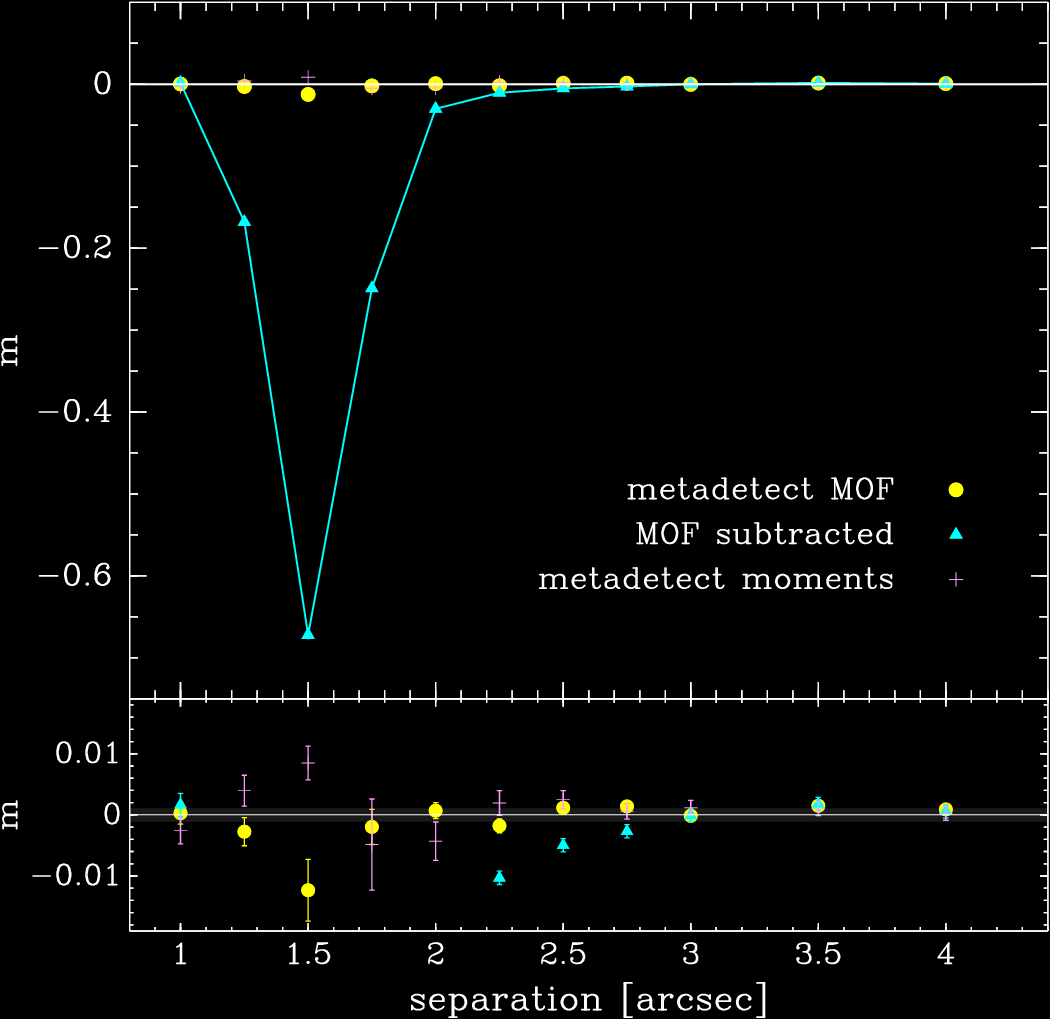
\includegraphics[width=\columnwidth]{pairs-mc-bdkpair-negate.png}
            \end{center}
        \end{column}
    \end{columns}
\end{frame}

\begin{frame}
    \frametitle{Metacalibration results for pair test}

    \setbeamerfont*{itemize/enumerate body}{size=\small}
    \setbeamerfont*{itemize/enumerate subbody}{parent=itemize/enumerate body}
    \setbeamerfont*{itemize/enumerate subsubbody}{parent=itemize/enumerate body}
 
    \begin{columns}
        \begin{column}{0.4\textwidth}
            \begin{itemize}

                \item Interpret as a shear-dependent detection bias.

                \item We can mitigate the effect empirically; I will explain
                    the other symbols later.

            \end{itemize}
        \end{column}
        \begin{column}{0.6\textwidth}
            \begin{center}
                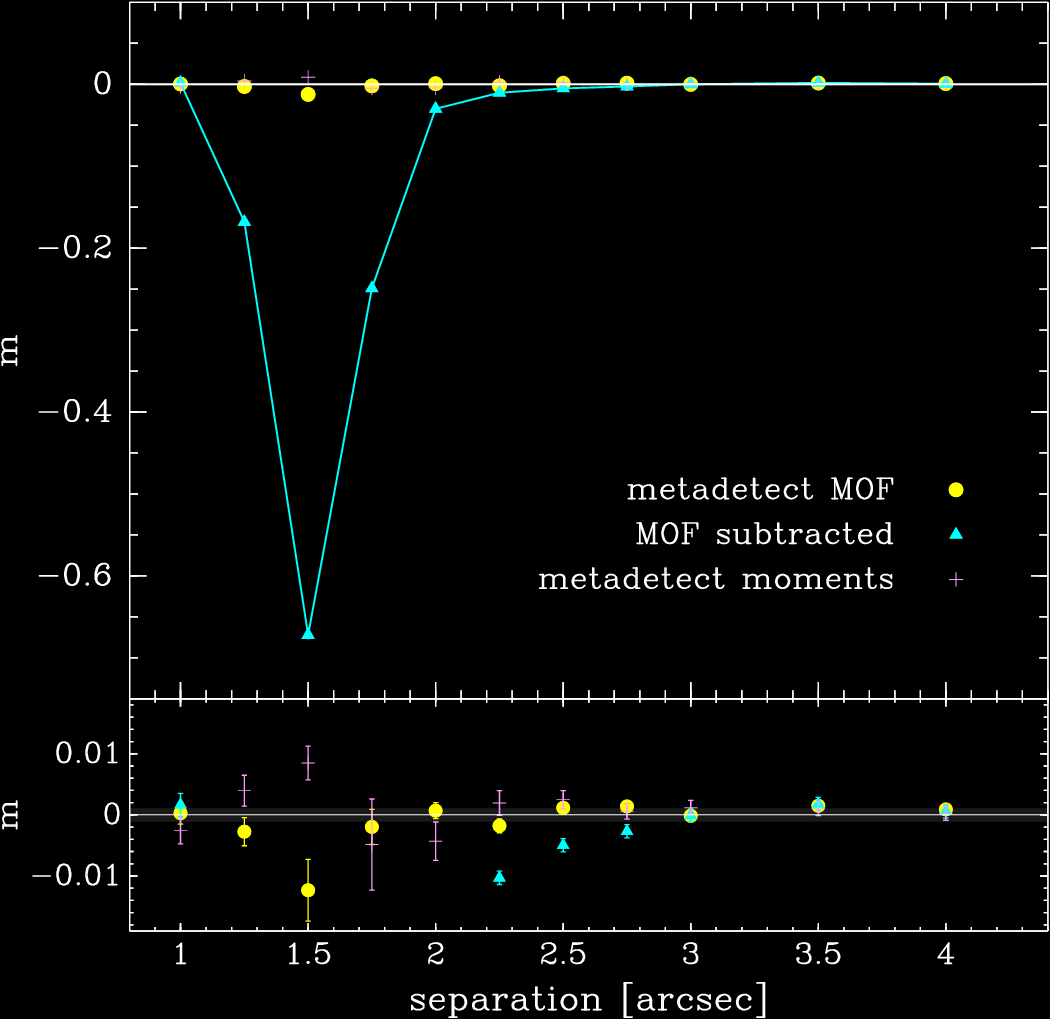
\includegraphics[width=\columnwidth]{pairs-mc-bdkpair-negate.png}
            \end{center}
        \end{column}
    \end{columns}
\end{frame}


\frame
{
    \frametitle{More Realistic Tests}

    \setbeamerfont*{itemize/enumerate body}{size=\normalsize}
    \setbeamerfont*{itemize/enumerate subbody}{parent=itemize/enumerate body}
    \setbeamerfont*{itemize/enumerate subsubbody}{parent=itemize/enumerate body}
 
    \begin{itemize}

        \item Same object types and survey parameters as the pair tests.

        \item Distribution of flux and size taken from the COSMOS catalogs.

        \item Noise appropriate for DES Y5

        \item sim1: \neff=10/sq arcmin for $S/N > 10$ and $T/T_{PSF} > 0.5$
            
        \item sim2: \neff=20/sq arcmin
            %acheived by just doubling the number of galaxies.
            %i.e. not by lowering the noise appropriately.

    \end{itemize}

}

\begin{frame}
    \frametitle{More realistic sims}
 
    \begin{columns}
        \begin{column}{0.5\textwidth}
            \begin{center}
                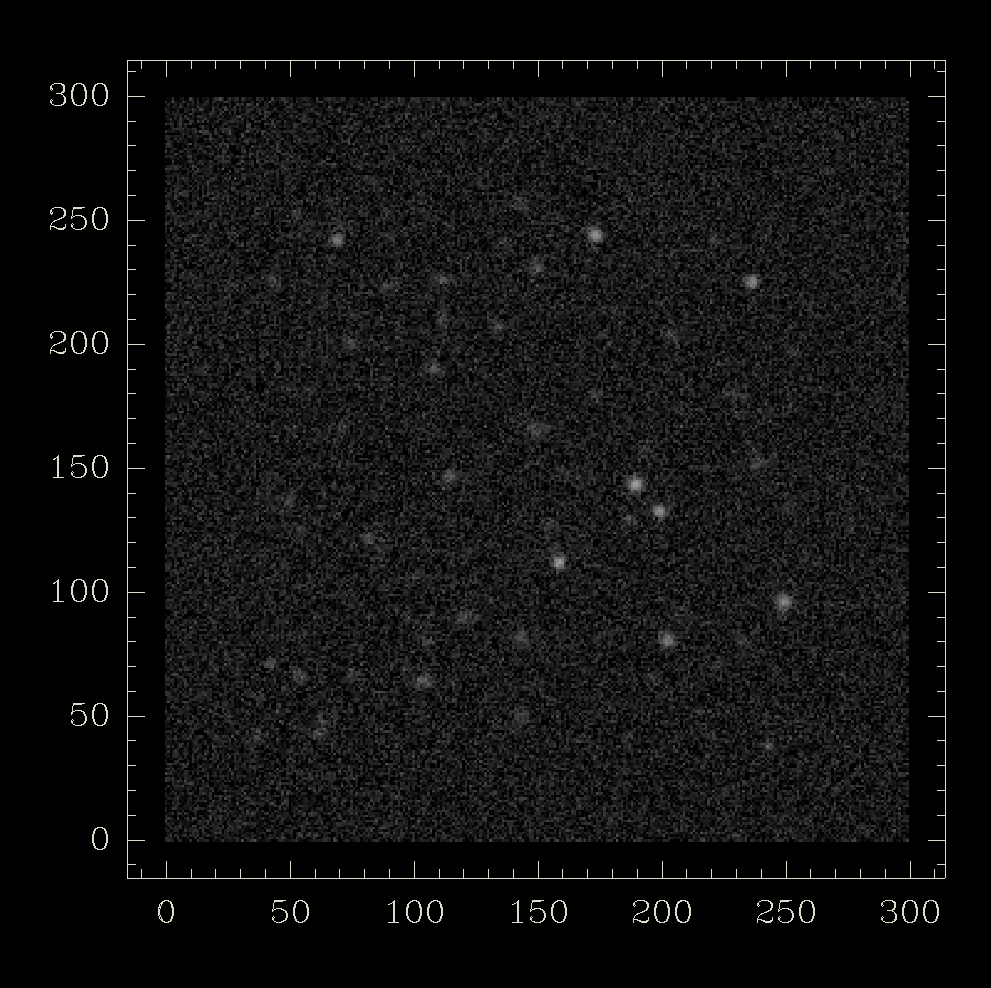
\includegraphics[width=\columnwidth]{10persqarcmin.png}
                \newline
                \neff=10/sq. arcmin
            \end{center}
        \end{column}
        \begin{column}{0.5\textwidth}
            \begin{center}
                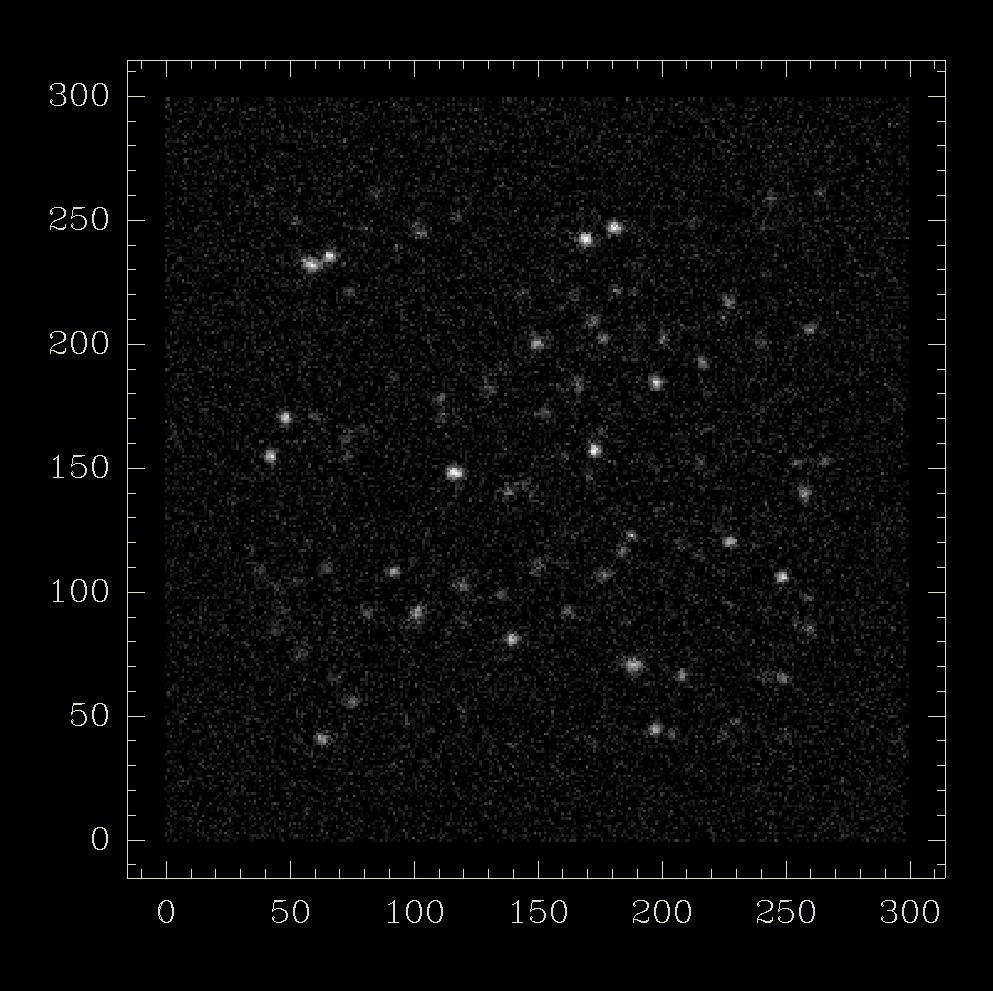
\includegraphics[width=\columnwidth]{20persqarcmin.png}
                \newline
                \neff=20/sq. arcmin
            \end{center}
        \end{column}
    \end{columns}
\end{frame}

\begin{frame}
    \frametitle{Metacalibration results for more realistic sims}

    \setbeamerfont*{itemize/enumerate body}{size=\small}
    \setbeamerfont*{itemize/enumerate subbody}{parent=itemize/enumerate body}
    \setbeamerfont*{itemize/enumerate subsubbody}{parent=itemize/enumerate body}
 
    \begin{table}
        \centering
        \begin{tabular}{|l|l|c|c|}
            \hline
            Sim & Method         & \snr\ Cut & m             \\
            %    &          &           & $[10^{-2}]$   \\
            \hline

            \hline
            \neff=10    & MOF+metacal    & \snr$ > 10$ & $XXX \pm XXX$  \\
            \neff=10    & MOF+metacal    & \snr$ > 15$ & $XXX \pm XXX$  \\
            \neff=10    & MOF+metacal    & \snr$ > 20$ & $XXX \pm XXX$  \\
            \hline
            \neff=20    & MOF+metacal    & \snr$ > 10$ & $XXX \pm XXX$  \\
            \neff=20    & MOF+metacal    & \snr$ > 15$ & $XXX \pm XXX$  \\
            \neff=20    & MOF+metacal    & \snr$ > 20$ & $XXX \pm XXX$  \\
            \hline

        \end{tabular}
        \caption{Bias in more realistic simulations.  In all cases a cut
            of $T/T_{PSF} > 0.5$ was also applied.
        \label{tab:mcal:deblending}}
    \end{table}


\end{frame}




\begin{frame}
    \frametitle{Results when \mcal\ includes the detection phase.}

    \setbeamerfont*{itemize/enumerate body}{size=\small}
    \setbeamerfont*{itemize/enumerate subbody}{parent=itemize/enumerate body}
    \setbeamerfont*{itemize/enumerate subsubbody}{parent=itemize/enumerate body}
 
    \begin{table}
        \centering
        \begin{tabular}{|l|l|c|c|}
            \hline
            Sim & Method         & \snr\ Cut & m             \\
            %    &          &           & $[10^{-2}]$   \\
            \hline

            \hline
            \neff=10    & metadetect+MOF    & \snr$ > 10$ & $XXX \pm XXX$  \\
            \neff=10    & metadetect+MOF    & \snr$ > 15$ & $XXX \pm XXX$  \\
            \neff=10    & metadetect+MOF    & \snr$ > 20$ & $XXX \pm XXX$  \\
            \hline
            \neff=20    & metadetect+MOF    & \snr$ > 10$ & $XXX \pm XXX$  \\
            \neff=20    & metadetect+MOF    & \snr$ > 15$ & $XXX \pm XXX$  \\
            \neff=20    & metadetect+MOF    & \snr$ > 20$ & $XXX \pm XXX$  \\
            \hline

        \end{tabular}
        \caption{Bias in more realistic simulations when \mcal\ includes
            the detection phase.  Deblending was performed using MOF. 
            In all cases a cut of $T/T_{PSF} > 0.5$ was also applied.
        \label{tab:mcal:deblending}}
    \end{table}


\end{frame}


\begin{frame}
    \frametitle{\mcal\ includes the detection phase and no deblending.}

    \setbeamerfont*{itemize/enumerate body}{size=\small}
    \setbeamerfont*{itemize/enumerate subbody}{parent=itemize/enumerate body}
    \setbeamerfont*{itemize/enumerate subsubbody}{parent=itemize/enumerate body}
 
    \begin{table}
        \centering
        \begin{tabular}{|l|l|c|c|}
            \hline
            Sim & Method         & \snr\ Cut & m             \\
            %    &          &           & $[10^{-2}]$   \\
            \hline

            \hline
            \neff=10    & metadetect+moments    & \snr$ > 10$ & $0.000 \pm 0.001$  \\
            \neff=10    & metadetect+moments    & \snr$ > 15$ & $0.000 \pm 0.002$  \\
            \neff=10    & metadetect+moments    & \snr$ > 20$ & $-0.004 \pm 0.003$  \\
            \hline
            \neff=20    & metadetect+moments    & \snr$ > 10$ & $0.002 \pm 0.001$  \\
            \neff=20    & metadetect+moments    & \snr$ > 15$ & $0.001 \pm 0.002$  \\
            \neff=20    & metadetect+moments    & \snr$ > 20$ & $XXX \pm XXX$  \\
            \hline

        \end{tabular}
        \caption{Bias in more realistic simulations when \mcal\ includes
            the detection phase.  No deblending was performed, 
            moments were measured using a circular Gaussian weight function.
            In all cases a cut of $T/T_{PSF} > 0.5$ was also applied.
        \label{tab:mcal:deblending}}
    \end{table}


\end{frame}


%\frame
%{
%    \frametitle{Fluxes: comparison of formula with simulation}
 
%        %\newline
%        $\Delta \sigma_p/\sigma_p = 0.10$
%    \begin{center}
%        \colorbox{white}{
%            \includegraphics[width=\columnwidth]{{cnoise-fwhm0.90-frac0.10-ntrial100000}.pdf}
%        }
%        \newline
%        (Sheldon, Armstrong, Huff, et al. in prep)
%    \end{center}


%}


\end{document}
